
% Example figure
\begin{figure}[H]
\centering
\setlength{\fboxrule}{2pt}
\setlength{\fboxsep}{0pt}
\fbox{
    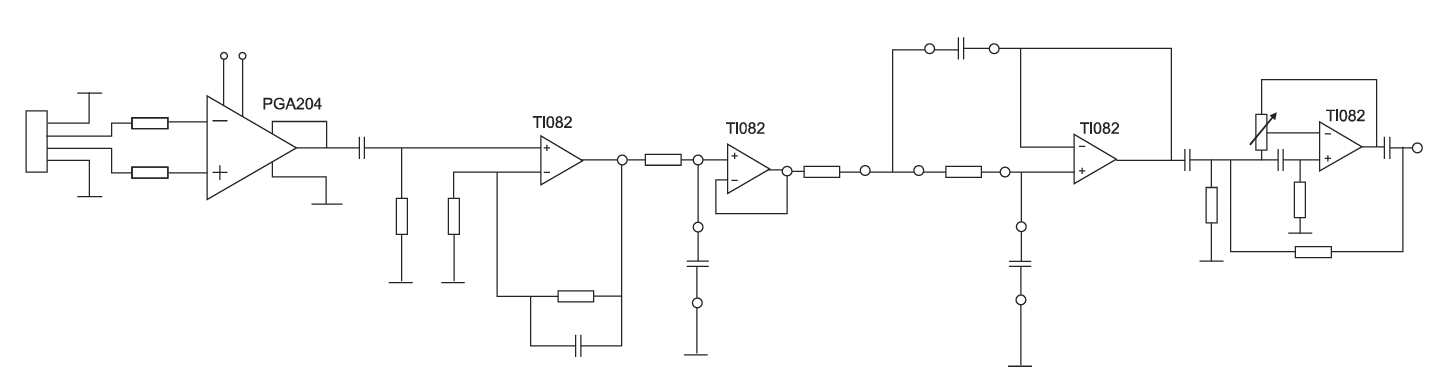
\includegraphics[width=1\textwidth]{figures/tor_pomiarowy.png}
}
\caption{Uproszczony schemat projektowanego toru pomiarowego.}
\end{figure}

% Example table
\begin{table}[H]
\centering
\begin{tabular}{|l|c|c|}
\hline
\textbf{} & \textbf{i = 1} & \textbf{i = 2} \\
\hline
a & 0,7560 & 0,9996 \\
\hline
b & 0 & 0,4772 \\
\hline
k & 1,323 & 1,414 \\
\hline
Q & - & 0,69 \\
\hline
\end{tabular}
\end{table}

% Example citation
Here is a citation to an article:
\cite{article_1}
Nosił wilk razy kilka, ponieśli i wilka\ldots

% xxx